\documentclass[15pt]{article}

% Language setting
% Replace `english' with e.g. `spanish' to change the document language
\usepackage[english]{babel}
\usepackage{graphicx}
\graphicspath{ {./images/} }
% Set page size and margins
% Replace `letterpaper' with `a4paper' for UK/EU standard size

\usepackage[letterpaper,top=2cm,bottom=2cm,left=3cm,right=3cm,marginparwidth=1.75cm]{geometry}

% Useful packages
\usepackage{amsmath}
\usepackage{graphicx}
\usepackage[colorlinks=true, allcolors=blue]{hyperref}

\title{TP3 Automatique}

\begin{document}
\maketitle

\begin{abstract}
\end{abstract}

\section{Commande de rotation d'un satellite}

a) $G(P) = \frac{Y(P)}{U(P)} $

$J\times \frac{d^2y}{dt^2} + \gamma \times \frac{dy}{dt} =U(p)$ 
\\
\\
$ Y(P) (JP^2 + \gamma P) = U(P)$
\\
\\
$G(P) = \frac{1}{JP^2 + \gamma P}$ \\

Le système est d'ordre 2. 



\subsection{}
a) 
$H(P) = \frac{KG(P)}{1+KG(P)} = \frac{\frac{1}{JP^2 + \gamma P}}{\frac{JP^2 + \gamma P + K}{JP^2 + \gamma P}} = \frac{K}{JP^2+\gamma P + K}$

c) 
$Y(P) = H(P) \times E(P) = \frac{K}{JP^2+\gamma P + K} \times \frac{\alpha}{P} = \frac{\alpha K }{ JP^3 + \gamma P^2 + KP} = \frac{\alpha K}{P(JP^2 + \gamma P + K)} = \frac{\alpha K }{JP(P-p_0)(P-p_1)}$
y(t) = $\alpha K \times (\frac{1}{p_0p_1} + \frac{e^{p_0t}}{(p_0)(-p_1+p0)} + \frac{e^p_1t}{p_1(-p_0 + p_1)})$

e) 
$p_0 = a+ib p_1 = a-ib$
$ 
y(t) = \alpha K \left( \frac{1}{(a+ib)(a-ib)} + \frac{e^{(a+ib)t}}{(a+ib)(-a+ib+a+ib)} + \frac{e^{(a-ib)t}}{(a-ib)(-a+ib+a-ib)} \right) $

f) \
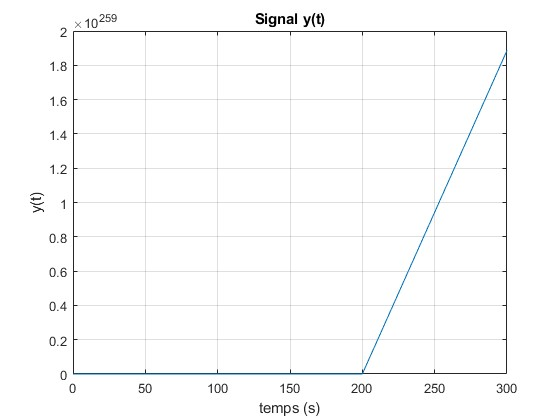
\includegraphics{untitled.jpg}


\end{document}
	
